\chapter{智能会话系统}{Toward Intelligent Dialgoue}

       本文研究的其中一个长远目标便是结合前文提到的各项自然语言处理和逻辑推理技术,构建一个能较好地与人交流沟通的智能会话系统,此系统将通过将接收到的人类话语转化成逻辑表达形式,并且结合系统本身的动机和情感状态,经过一定的解析和逻辑推理,从而得到想表达的内容的逻辑表达形式,最后将这些逻辑表达式再转化成自然语言回应给谈话对象。
       本章将重点介绍这样的智能会话系统(以下简称“CogDial”)的系统架构,该系统基于前面章节描述的自然语言理解和自然语言生成的相关技术,并通过OpenCog的核心子系统(主要是PLN和OpenPsi)来控制其对话结构和表达方式。该CogDial系统能够灵活地理解和处理具有不同程度的复杂性和智能性的人类言语行为。创建一个完全符合人类标准的人工智能对话系统无疑是一个精彩的挑战,但似乎在当前的科学技术水平下,也无疑是一个非常困难的研究项目。 相对于目前主流的基于规则或者基于统计的对话系统,我们这里提出的CogDial架构引入目标驱动的逻辑推理和情感控制等,显然表现更智能些,但还不足以完全达到符合人类智能标准。这样一个介于目前相关研究水平和完全人类水平之间的对话系统可以看做是朝构建更人性化的会话系统的一个重要步骤,或者看做是使用更可行的研究方法在人机对话系统集成更多的功能,而不是一味地去盲目追求达到人类水平的目标。本着这样的理念,说的更具体点,我们CogDial的目标不是精确类似人类的对话,而是具备通用认知能力、情感表达能力、能合理结合语用和经验的智能会话系统。
         CogDial的初步预期目标主要是实现面向游戏角色和人性机器人的对话系统,但同样的研究思路也完全能应用在基于文本的对话系统,例如智能对话搜索接口。我们分阶段来实现这样的系统,从一个相对小而简单的系统为起点,通过不断改进和完善,以及系统本身的自学习和认知能力,最终实现一个在一定程度上接近人类水平的系统。目前,我们的系统还没有达到最终的水平,但基本框架已经到位。除此之外,我们构建了一个基于超图匹配的问答系统的原型,该问答系统使用前文提到的自然语言处理将自然语言转换成以超图表达的语义逻辑形式,利用基于超图匹配的动态编程算法,从而在问答语料库中找到最适合问题的答案来响应用户查询。

\section{基于Psi的对话控制}{Applying the Psi model to Dialogue Control}
构建一个完整能运作的智能对话系统,除了需要前文提到的各项关键技术, 宏观规划(以下称为“Marcoplanning”)也是必不可少的部分。从言语行为理论来看,宏观规划可以看成是一个可以规划以下两点的工具:1)在哪个时间点发生哪些言语行为,2)使用哪些内容去封装这些言语行为。宏观规划更多的是从语用和推理方面出发,淡化语义或语法(或者音韵词汇等)的限制。
      CogDial智能对话系统中的宏观规划涉及到了OpenCog中的情感动机计算模型OpenPsi,因此,在本节我们会首先给出OpenPsi的高度概括,侧重于介绍其在自然语言会话系统中应用的可行性。

\subsection{Psi模型中的动机行为}{The Psi Model of Motivated Action}
       为了更好的解释OpenPsi,我们需要从Psi和MicroPsi谈起,Psi是由德国心理学家Dietric Dorner提出的情感认知动机理论模型 \cite{Dorner2002},将情感与智能体的需求和动机相联系。{\bf MicroPsi} \cite{Bach2009},是一个基于Psi理论的一个开源的智能认知体系结构,实现了Psi理论中的动机、情感以及智能的关联模型,并在一些实用控制应用以及简单虚拟世界里的智能体上进行测试。MicroPsi在全面性以及神经科学和心理学依据方面做得非常出色,但是该认知体系结构在可扩展性上存在不少问题, \cite{EGI1}中,有人认为,MicroPsi目前使用的算法在学习和推理上不大可能被扩展或规模化。
       OpenCog受Psi理论中的动机和情感模型的启发,借鉴了很多MicroPsi的基本实现方法,实现了类似的情感动机模型OpenPsi。虽然OpenPsi和MicroPsi在一定程度上很相似,但两者 还是存在着很大的不同。比如,两者使用了完全不同的知识表达方式, MicroPsi则使用了类似神经元的“quad”来表示知识,每一个quad包括5个神经元,其中一个是核心神经元,其他4个描述与核心神经元的“前/后”或者“部分/整体”等关系。OpenPsi使用了本文第三章中介绍的OpenCog的基于超图的知识表示,显然是一种更灵活和通用的知识表示方式。 MicroPsi目前还是注重底层的智能的实现,还未开始着手高层的智能处理,如自然语言处理和抽象逻辑推理。
       
在本节对Psi和MicroPsi的概述中,我们主要介绍其在OpenCog被应用的部分,主要是处理动机、行为和目标的框架模型。

Psi理论中的动机机制可参考图\ref{fig:Psi},从下往上看,不难发现Psi的动机机制从能激发智能体的需求出发。对于动物来说,该需求可以是食物、水、保护自己的孩子、社交需求、求新等等;对于智能机器人来说,该需求可能是电源、 完整性(保护身体完整Integrity)、确定性(了解和熟悉环境的需求Certainty)、认知需求、心里成长等等;对于智能对话系统来说,该需求可以包括收集相关信息、取悦谈话对象、使会话保持新颖不枯燥等。

Psi理论特别指出了两种相当抽象的需求,并认为他们是心理学上的最基本需求[见图XX]


\begin{itemize}
\item 能力需求(Competence):智能体能有效实现某种强烈欲望的需求
\item 确定性需求(Certainty):智能体了解和熟悉环境的需求
\end{itemize}

每种需求都有一定的偏好范围或目标范围,随着时间和环境(包括智能体自身)的不断变化,智能体的需求也在不断地变化。 当需求水平落在相应的目标范围时,
称作该需求被满足,否则需求不被满足。我们可以将智能体视为一个目标驱动的
系统,其主要任务就是尽可能让所有这些需求都被满足。而当某一需求不被满足
时,智能体会有一种试图将该需求水平恢复到偏好范围内的愿望,这种愿望便构
成了动机。

\begin{figure}[htb]
\centering
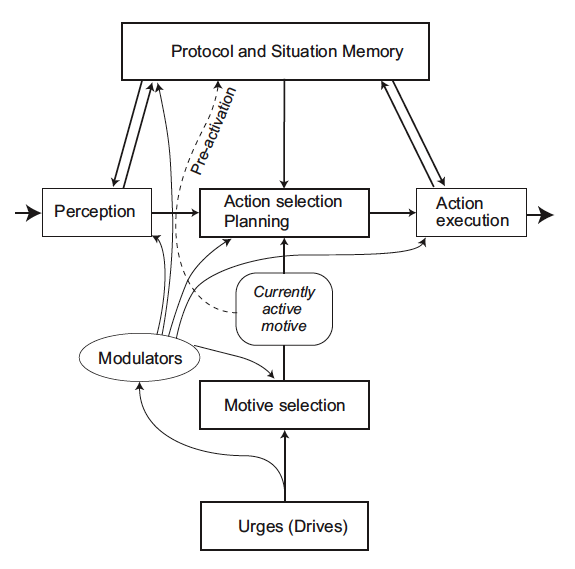
\includegraphics[width=11cm]{figures/Psi.png}
\caption{High-Level Architecture of the Psi Model}
\label{fig:Psi}
\end{figure}

%%%%%%%%%%%%%%%%%%%%%%%%%%%%%%%%
\subsection{Emotion and Personality in the Psi Model}{Emotion and Personality in the Psi Model}
%%%%%%%%%%%%%%%%%%%%%%%%%%%%%%%%

%%%%%%%%%%%%%%%%%%%%%%%%%%%%%%%%
\section{OpenPsi:OpenCog中的基于Psi的情感计算模型}{OpenPsi: Psi-Based Motivated Action in OpenCog}
%%%%%%%%%%%%%%%%%%%%%%%%%%%%%%%%

We now describe how Psi-based structures and dynamics are integrated into OpenCog, to provide a framework for motivated action that supplies the macroplanning component of our CogDial dialogue system.

本节将介绍如何在OpenCog中集成基于Psi的

%%%%%%%%%%%%%%%%%%%%%%%%%%%%%%%%
\subsection{Action Selection in OpenCog}{Action Selection in OpenCog}
%%%%%%%%%%%%%%%%%%%%%%%%%%%%%%%%

As Stan Franklin likes to point out \cite{Franklin1995}, the essence of an intelligent {\it agent} is that it does things; it takes {\it actions}.  The particular mechanisms of action selection in OpenCog are a bit involved and are described in depth in \cite{EGI2}; in this chapter we will give the basic idea of the action selection mechanism and then explain how a variant of the Psi model is used to handle {\it motivation} (emotions,  drives, goals, etc.) in OpenCog, including the guidance of action selection.

The crux of OpenCog's action selection mechanism  is  as follows

\begin{itemize}
\item the action selector chooses procedures that seem likely to help achieve important goals in the current context
\begin{itemize}
\item {\it Example:} If a highly important, current goal is to please the conversation partner, and the conversation partner has asked a question, then answering the question may be a procedure estimated as highly likely to achieve the "please the conversation partner" goal
\end{itemize}
\item to support the action selector, the system builds implications of the form $Context \& Procedure \rightarrow Goal$, where Context is a predicate evaluated based on the agent's situation
\begin{itemize}
\item {\it Example:} If Bob has asked the agent (the dialogue system) to compose a certain kind of paragraph, and it knows that Bob is very insistent on being obeyed, then  implications such as
 \begin{itemize}
 \item ``Bob instructed to do X''  and ``do X''  $\rightarrow$ ``please Bob''  $<.9,.9>$
 \end{itemize}
 will be utilized
\item {\it Example:} If the agent wants to make its conversation partner believe a statement X, then implications such as
 \begin{itemize}
 \item ``tell Bob the key reasons why I believe X is true''  and ``I want to convince Bob that X is true''  $\rightarrow$ ``satisfaction''  $<.9,.9>$
 \end{itemize}
 will be utilized 
\end{itemize}
\item the truth values of these implications are evaluated based on experience and  inference
\begin{itemize}
\item {\it Example:} The first example could be evaluated based on experience, by assessing it against remembered episodes involving Bob giving instructions
\item {\it Example:} The same example could be evaluated based on inference, using analogy to experiences with instructions from other individuals similar to Bob; or using things Bob has explicitly said, combined with knowledge that Bob's self-descriptions tend to be reasonably accurate
\end{itemize}
\item Importance values are propagated between goals using economic attention allocation (and, inference is used to learn subgoals from existing goals).  This is an aspect we have not yet explored in practice in CogDial, but we believe it will be helpful for achievement of more sophisticated dialogue behavior.
\begin{itemize}
\item {\it Example:} If Bob has told the agent to do X, and the agent has then derived (from the goal of pleasing Bob) the goal of doing X, then the ``please Bob''  goal will direct some of its currency to the ``do X''  goal (which the latter goal can then pass to its subgoals, or spend on executing procedures)
\end{itemize}
\end{itemize}

%%%%%%%%%%%%%%%%%%%%%%%%%%%%%%%%
\subsection{Psi in OpenCog}{Psi in OpenCog}
%%%%%%%%%%%%%%%%%%%%%%%%%%%%%%%%

%%%%%%%%%%%%%%%%%%%%%%%%%%%%%%%%
\subsection{Goals in OpenCog}{Goals in OpenCog}
%%%%%%%%%%%%%%%%%%%%%%%%%%%%%%%%

%%%%%%%%%%%%%%%%%%%%%%%%%%%%%%%%
\subsection{Execution Management}{Execution Management}
\label{Execution Management}
%%%%%%%%%%%%%%%%%%%%%%%%%%%%%%%%

%%%%%%%%%%%%%%%%%%%%%%%%%%%%%%%%
\section{The CogDial Dialogue System Architecture}{The CogDial Dialogue System Architecture}
%%%%%%%%%%%%%%%%%%%%%%%%%%%%%%%%

下面我们来介绍基于上述的目标控制体系的智能会话系统CogDial的系统框架。目前该系统只能处理英文对话,接下来章节中的对话的例子基本按照英文的习惯举的例子,可能不太适合中文的习惯,但是该系统的所采用的技术和理论基础都是完全适合中文的。CogDial主要采用了以下技术:

\begin{itemize}
\item  基于OpenPsi以及相关OpenCog机制的宏观规划(Macroplanning)
\item  本文第4章描述的句法分析和语义关系及逻辑关系抽取的自然语言理解技术
\item  本文第5章描述的微观规划(Microplanning)和表层生成的自然语言生成技术
\item  专门设计的符合智能会话系统的“言语行为规划器”集合,这些言语行为规划器将用于:
\begin{itemize}
    \item 在OpenPsi的控制机制下,结合当前的语境,激活相应的言语行为规划器
    \item 收集相关内容,生成能关联Microplanner的Atoms
    \item  调用一系列的认知机制(包括用于逻辑推理的PLN),选择相关的Atoms发送到Microplanner
\end{itemize}
\end{itemize}

%%%%%%%%%%%%%%%%%%%%%%%%%%%%%%%%
\subsection{针对对话控制的OpenPsi的配置}{Configuring OpenPsi for Dialogue Control}
%%%%%%%%%%%%%%%%%%%%%%%%%%%%%%%%

基于Psi的基本框架,我们选择了以下的具体需求用来指导我们的对话系统的行为:
\begin{itemize}
\item 社交需求(Affiliation):与他人互动,希望被其他成员接纳的需求;取悦谈话对象可以视为此目标的一个特例
\item 能力需求(Competence):通过对话达到某种目标的需求,衡量言语表达方式的指标
\item 确定性需求(Certainty):智能体对自身语境的了解需求,特别是对目标的了解需求
\item 新颖性需求(Novelty):维持智能的会话而不是简单重复的问答会话。
\end{itemize}

CogDial中的对话控制主要通过不同的需求来选择相应的言语行为规划器,因此,在选择言语行为规划器前,我们需要知道当前状态下上述每种需求的被满足的程度。鉴于目前的CogDial系统的有限能力,为了能更好地实现一个面向集成认知体系的智能会话系统框架,我们将上述的几项需求做了更具体化的定义:

\begin{itemize}
\item 社交需求(Affiliation):我们对该需求进行了下面三种满足程度:
\begin{itemize}
\item 当对话系统正在与人或者其他智能体进行会话时,该需求在一定程度上被满足;
\item 当系统正与多个人或智能体进行会话时,该需求被满足的程度提升;
\item  当该系统的会话内容都属于积极向上的时候(通过情感分析技术实现),该需求被满足的程度达到最高。
\end{itemize}
\item 能力需求(Competence):此项需求需要通过OpenCog来评估。简单来说,对每一个目标,OpenCog记录着会话系统在过去完成该项目标的程度,然后根据当前的不同目标所占的权重,我们可以通过以下公式估算该需求被满足的程度(首先针对每一个目标,计算目标权重*能达到该目标的概率,然后求总)。当然计算目标被完成的程度,还应该考虑实现目标的语境等因素,目前我们的系统更注重构建一个智能会话系统框架,因此在语境无关的假设下来衡量目标被实现的程度。
\item 确定性需求(Certainty):如果会话系统正在和一个陌生人对话,或者系统无法理解大量被提及的单词或概念,那么当前的确定性需求被满足的程度就会降低。如果系统获取了新的可靠知识,那么该需求被满足的程度就会增加。
\item 新颖性需求(Novelty):我们定义了以下几种方式来增加智能绘画系统对新鲜度需求的满足程度值:
\begin{itemize}
\item 多和不同的人类或智能体会话;
\item 谈论新的话题或引入新的词汇和概念;
\item 学习新的可靠信息( OpenCog推理得出的新的置信度高的知识存储的载体原子(Atoms))
\end{itemize}
\end{itemize}

基于上述目标需求的智能会话系统,除了需要结合前文所述的OpenPsi的框架理论,以及本文描述的自然语言理解和生成的相关工具之外,还需要有以下模块:
\begin{itemize}
\item 制定一组能被特定目标需求激活的对话控制程序
\item 建立目标和相应去实现目标的行为之间的关联,可通过相关规则来实现,也可以通过强化学习来实现,我们系统框架采用两种结合的方法,但目前的系统还是以规则关联为主。
\end{itemize}
  

%%%%%%%%%%%%%%%%%%%%%%%%%%%%%%%%%%%%%%%%%%%%%%%%%%%%%%%%%%%%%%%
\subsection {言语行为规划器}{Speech Act Schema}
\label{sec:SAS}
%%%%%%%%%%%%%%%%%%%%%%%%%%%%%%%%%%%%%%%%%%%%%%%%%%%%%%%%%%%%%%%

“言语行为规划器”(Speech Act Schema)是CogDial的一个核心设计, 每个言语行为规划器里包含一种特定的言语行为(Speech Act),以及与该言语行为对应的特定的认知行为(Cognitive Procedure)。每种言语行为规划器都能在不同情况下被激发调用。对于言语行为规划器的选择,我们采用OpenCog中的OpenPsi的动机驱动模块来执行。

    CogDial的总体规划是针对本文第 \ref{chap:litreview}章综述里提到的42种SWBD-DAMSL言语行为 \cite{Twitchell2004},实现相应的言语行为规划器。 CogDial目前只实现了42种中的部分言语行为对应的言语行为规划器。另一方面,CogDial中的言语行为规划器的设计也绝不局限于这42种言语行为,CogDial实现了一些言语行为规划器能对应这42种中的某两种或多种言语行为,比如我们利用真值回答规划器(TRUTH VALUE ANSWER schema)来同时关联其中的YES QUESTION和NO QUESTION,从而可以将一般疑问句的回答根据真值的大小延伸到“可能”“不确定”“可能不”等,而不仅仅是局限于回答“是”或者“不是”。CogDial还根据智能体的具体情况拆分了这42种中的某些言语行为,例如,我们针对言语行为“STATEMENT” 实现了两个不同的言语行为规划器:回应声明以及智能体自发的用于表达其自身状态和想法等的声明。

总的来说,本文虽然没有完全照搬SWBD-DAMSL的言语行为分类,但是,该分类体系是来源于对大量人类会话的进行具体分析后的实验结果,也在具体的会话分析和抽象的言语行为理论之间架起了桥梁,使得抽象的言语行为理论在机器上实现变得可行,因此,SWBD-DAMSL的言语行为分类体系还是很有借鉴价值的。

要实现上述的言语行为规划器,每一个言语行为都会引发一个相应的认知行为,也就是说,每一个言语行为都会触发调用一段程序;而这样的机制正好符合OpenCog里的 GroundedSchemaNode的用法。GroundedSchemaNode是OpenCog的超图知识库里的一种节点类型,通常被封装在ExecutionOutputLink里,连接着一段代码(一般情况下是Scheme或者Python编写的代码)的名称。该代码可以通过ExecutionOutputLink被触发和执行。因此,鉴于这样的执行机制,我们可以通过对每个言语行为规划器定义一个GroundedSchemaNode来实现言语行为规划器。这样的设计方案可以减少冗长复杂的代码块,而直接通过OpenCog中统一又通用的Atomspace的基本操作方法来管理和执行复杂的言语行为规划器。另外,这样的机制也能很容易调用知识库Atomspace之外的复杂程序,从而得到很好的扩展性,也为言语行为规划器的扩展研究搭建了个很好的平台。例如,我们可以通过调用外部程序将逻辑推理系统PLN的前向或者后向推理应用到言语行为规划器中,使其能实现自适应学习,不断完善言语行为规划器。本文后面会进一步讨论这样的扩展。

每一个言语行为规划器的输入是一个被叫做对话节点(DialogueNode),DialogueNode是可以表示一方或者多方之间的会话交互的节点类型。DialogueNode可以有不同话语节点(UtteranceNodes)作为成员,在实现方式上,DialgoueNode通过MemberLinks指向不同的UtteranceNodes。而UtteranceNode则可以关联以下不同类型的节点:
\begin{itemize}
\item 关联一个或多个文本节点(TextNode)、句子节点(SentenceNode)或者短语节点(PhraseNode),则表示输入的话语内容来自一个或者多个文本、句子或者短语。
\item  关联一个声音节点(SoundNode),则表示该话语来自外界声音。
\item  关联指向说话者的Link。
\item  关联指向对话语的补充信息的Links,这些补充信息可以是该话语的言语行为类型、与该话语相联系的情感等。
\item  关联指向产生话语的言语行为规划器,用于响应是什么触发该话语。
\item  关联一个或多个解析节点(InterpretationNode),这些解析节点可以是用来解析话语的语义和语用信息。
\end{itemize}

言语行为规划器的输出是连接了一系列相关联Atoms的SetLink,该输出会送入本文\ref{chap:generation}中描述的微观规划和表层生成等工具,从而产生相应的自然语言来回应输入的内容。言语行为规划器还会将输出的话语关联到产生该话语的DialogueNode,这样不仅仅是记录了会话的内容,还能用于智能体的强化学习和提高智能体的各种需求的满足度。
下面通过一个例子来解释上述的实现过程。假设有下面的简单对话:
\begin{verbatim}
Ruiting: How are you doing?
CogDial: I am fine
\end{verbatim}
这个简单的对话可用以下的Atoms来表示:

{\tt\begin{small}\begin{lstlisting}

MemberLink
	UtteranceNode [555]
	DialogueNode [123]
	
MemberLink
	UtteranceNode [666]
	DialogueNode [123]
	
EvaluationLink
	PredicateNode "say"
	ConceptNode "Ruiting"
	UtteranceNode [555]

EvaluationLink
	PredicateNode "say"
	ConceptNode "me"
	UtteranceNode [666]
		
EvaluationLink
	PredicateNode "Textual Content"
	UtteranceNode [555]
	SentenceNode "How are you doing?"
	
EvaluationLink
	PredicateNode "Textual Content"
	UtteranceNode [555]
	SentenceNode "I am fine."
	
EvaluationLink
	PredicateNode "Utterance Type"
	UtteranceNode [555]
	ConceptNode "Interrogative"
	
EvaluationLink
	PredicateNode "Utterance Type"
	UtteranceNode [666]
	ConceptNode "Declarative"
	
AtTimeLink
	UtteranceNode [555]
	TimeNode "22:15:33 12/06/2014"
	
AtTimeLink
	UtteranceNode [666]
	TimeNode "22:15:47 12/06/2014"
	
EvaluationLink
	PredicateNode "Interpretation"
	UtteranceNode [555]
	InterpretationNode [22]
	
EvaluationLink
	PredicateNode "Interpretation"
	UtteranceNode [666]
	InterpretationNode [33]
	
	
MemberLink
	EvaluationLink
		PredicateNode "doing"
		ListLink
			ConceptNode "you"
			VariableNode "var1"
	InterpretationNode [22]
	
	
MemberLink
	InheritanceLink
		ConceptNode "I"
		ConceptNode "fine"
	InterpretationNode [33]
	
ExecutionLink
	GroundedSchemaNode "polite_banter.scm"
	ListLink
		UttteranceNode [555]
		DialogueNode [123]
	UtteranceNode [666]

\end{lstlisting}\end{small}}

其中的命题也可以有多种选择,例如:

{\tt\begin{small}\begin{lstlisting}
EvaluationLink
	PredicateNode "Conversation Partner"
	DialogueNode $D
	$X
\end{lstlisting}\end{small}}

该命题为真,当且仅当,$X是$D其中一个话语的发言人。


\section{Initial Speech Act Schema and their Linkage to Goals and Contexts}{Initial Speech Act Schema and their Linkage to Goals and Contexts}

在\cite{Twitchell2004}, 中,Twitchell和Nunamaker根据Searl的言语行为理论的经典分类,在对大量的人类会话进行经验分析后,将言语行为细分为42种。虽然此分类体系很有理论研究价值,但在实验过程中,考虑到实用智能会话系统的语境等因素,我们对这42种言语行为做了稍微调整,同时也在CogDial中添加了一些SWBD-DAMSL研究中没有出现言语行为。

即使在有明确的言语行为类型的情况下,仍然有很多种方法去构建一个智能会话系统。CogDial根据多个广泛的可扩展目标制定一些特定的设计决策,在这些决策基础上,系统能通过自适应学习方法自动改进,为能跳出传统的对话系统的研究方法搭建一个基础平台。为了搭建这样的系统,需要考虑的第一点是,对于每一个言语行为,都有相应的固定形式的认知内容被触发,也有相应的习惯性表达方式来表达该认知内容。

如果在类似的言语行为类型分类基础上构建一个简单的“聊天机器人”,一般通过更简单,不用加入很多认知处理,针对每个言语行为类型,输出直接的具体的话语,也同样能达到类似的效果。例如,对于言语行为类型Agree,可以编写简单的程序使智能体输出“同意(Agree)”或者“是的,我同意(Yes, I agree)”。目前,“聊天机器人”的概念很模糊。我们这里提到的“聊天机器人”范围也很广,可以是完全基于模板匹配的聊天机器人ELIZA\cite{Weizenbaum1966},也可以是具有一些推理能力但是基本忽略语义理解的众所周知的Siri。但关键的一点是,我们设计的CogDial系统,是本着该系统能“理解”自己在说什么的理念,也就是说,该系统所产生的话语来自于内部的语义关系图,且该语义关系图和系统知识库中的其他语义关系图之间有着丰富的语义关系。我们希望系统能在一定程度上更深地“理解”自己在说什么,而不是只生成它不理解的字符串。在某些情况下,在不理解的情况下破口而出一些话语,尤其是习惯用语,也是可以接受的(其实人类有时候也会无意识地这么做),但这并不是大部分情况。

在CogDial系统的设计中,每一个言语行为都需要下列几项内容与之相应:
\begin{itemize}
\item 相应的目标和语境二元组(goal,context),表明何时该言语行为会被触发。
\item 相应的能生成相关信息的程序,产生由该言语行为引起的要传递给谈话对象的信息。
\item 一个或多个相应的“语义模板”,表明由该言语行为引发的相关认知内容。
\item 连接上述语义模板所在的Atoms和特定的句子实现的Atoms的Links,用于传送到Microplanning,从而生成相应的话语。
\end{itemize}

这样一来,通过编写一些抽象的语义形式和特定的会话习惯之间的匹配模式,便能构建出一个具有一定合理功能的智能会话系统,当系统学习了用不同的更复杂的表达方式去实现抽象的语义形式后,也就能在更大程度上“理解”会话内容。此外,这些抽象的语义形式除了与言语行为和目标需求相关联,还和其他不同的认知内容相关联,因此,系统会随着经验的增长而趋向成熟。
假设任何言语行为被触发都能增加下面表达式中的EvaluationLink的真值:
 {\tt\begin{small}\begin{lstlisting}
EvaluationLink
	PredicateNode "Currently Having Conversation"
	TimeNode T
\end{lstlisting}\end{small}}
    其中,“T”表示当前时间。又假设上面表达式中的EvaluationLink和系统中多个顶层目标有关联(该假设对于某些应用也不总为真,那么在这样的情况下,这些不为真的关联的链的权重会根据具体情况被调为适当的值),也就是说,该系统能看到会话行为带来的价值。 因为每个言语行为都蕴含着这个EvaluationLink,所以每个言语行为都会影响系统的目标实现。一些言语行为会通过持续进行对话从而超标完成某个系统目标。这样的言语行为会在后面章节详述。
    下面会给出一些具体的例子进一步解析前面几段提到的Atoms。
 {\tt\begin{small}\begin{lstlisting}
ImplicationLink <.5>
	EvaluationLink
		PredicateNode "Currently Having Conversation"
		TimeNode $T
	EvaluationLink
		PredicateNode "Increase Knowledge"
		TimeNode $T
\end{lstlisting}\end{small}}
上述超图片段表明,维持对话能在一定程度上满足系统目标“增长知识”,ImplicationLink的初始权重设为0.5,表明“当前有会话”蕴含系统目标“增长知识”只有0.5的概率。这个权重会随着系统的经验而改变,也会通过其关联的其他节点和链的具体情况推算得来。例如:
 {\tt\begin{small}\begin{lstlisting}
ImplicationLink <.1>
	ANDLink
		EvaluationLink
			PredicateNode "Currently Having Conversation"
			TimeNode $T
		EvaluationLink
			EvaluationLink "DialoguePointer"
			PredicateNode "Currently Having Conversation"
			DialogueNode $D
		EvaluationLink
			PredicateNode "Conversation Partner"
			ConceptNode "Bob"		
	EvaluationLink
		PredicateNode "Increase Knowledge"
		TimeNode $T
\end{lstlisting}\end{small}}

上面的超图片段表明,当进行对话的对象是Bob的时候,只有0.1的概率能实现系统目标“增长知识”。
{\tt\begin{small}\begin{lstlisting}
ImplicationLink <1>
	ExistsLink $G, $S, $O, $U, $D
		ANDLink
			MemberLink
				GroundedSchemaNode $G
				ConceptNode "Speech Act Schema"
			AtTimeLink
				TimeNode $T
				ExecutionLink
					GroundedSchemaNode $G
					$S
					$O
			MemberLink
				UtteranceNode $U
				DialogueNode $D
			EvaluationLink
				PredicateNode "Textual Content"
				UtteranceNode $U
				SentenceNode $O
			AtTimeLink
				TimeNode $T
				EvaluationLink
					PredicateNode "Currently active"
					DialogueNode $D			
		EvaluationLink
			PredicateNode "Currently Having Conversation"
			TimeNode $T
\end{lstlisting}\end{small}}

上面的例子说明,如果一个言语行为规划器被执行,当前的对话节点(DialogueNode)$D$会关联一个谓词“当前活跃”,表明$D$出于活跃状态, 那么“当前有会话”的目标被实现。

 {\tt\begin{small}\begin{lstlisting}
MemberLink
	GroundedSchemaNode "answer_yes.scm"
	ConceptNode "Speech Act Schema"
\end{lstlisting}\end{small}}

接下来的例子演示了言语行为如何与目标关联:

 {\tt\begin{small}\begin{lstlisting}
ImplicationLink <.8>
	ExistsLink $S, $O, $U, $D
		ANDLink
			AtTimeLink
				TimeNode $T
				ExecutionLink
					GroundedSchemaNode "answer_yes.scm"
					$S
					$O
			MemberLink
				UtteranceNode $U
				DialogueNode $D
			EvaluationLink
				PredicateNode "Textual Content"
				UtteranceNode $U
				SentenceNode $O
			AtTimeLink
				TimeNode $T
				EvaluationLink
					PredicateNode "Currently active"
					DialogueNode $D			
		EvaluationLink
			PredicateNode "Please Conversation Partner"
			TimeNode $T
\end{lstlisting}\end{small}}

上面的例子表明言语行为规划器“肯定回答”(”Answer Yes”schemma)可以用于增加实现“取悦谈话对象”目标的幅度值,超越了谈话对象因单纯继续对话而被取悦的程度。

许多言语行为规划器都会有不同的清晰表达相关语义内容的方式。比如说,一般会话的开头,可以说“你最近状态怎么样?”(”What has your state been recently?”),或者“你最近都忙什么?”(“What have you been doing?”) 等,而类似这样的语义内容很容易约定俗成地被说成“最近怎么样?”(“What’s up?”)。对于机器来讲,如果对话系统直接问 “What’s up?” 当然也没问题,但是有必要使系统知道 “What’s up?”只是其他两种说法或者 “what are you thinking about?“的一种约定俗成的简约说法。系统会根据智能体的不同个性对每种不同的说法一个相应的权值。

一般来说,会存在很多的“个性参数”影响着多种言语行为。在CogDial的实现过程,我们针对那些对对话影响较大的关键特性(我们称为“对话特征”(Dialogue-trait))创建相应的概念节点(ConceptNode),比如:习惯用语(Idiomaticity)、非正式(Informality)、精确(Precision)、累赘(Wordiness)、开放(Openness)。用来表示由言语行为规划器产生的具体话语的SetLink,将以不同的权重与这些表示不同对话特征的ConceptNode相连。例如,表示“I dunno”的SetLink将以较高的权重与“Informality”以及“Idiomaticity”关联,以较低的权重与“Precision”“Wordiness”关联。这些对话特征的参数可以在对CogDial设置基本参数的时候根据不同的需求人为设计。也可以在对话过程中根据谈话对象的喜好来自适应地调整。

综上所述CogDial的整个设计方案中,需要人工参与的部分包括:
\begin{itemize}
\item 自然语言理解流水线中的提到的规则(最终会被我们正在研究的无监督语言学习所取代,本文第9章有更详细的阐述)
\item OpenPsi中的顶层目标
\item 不同的言语行为所引发的不同认知过程。目前这些过程是在与GroundedSchemaNode绑定的相应Scheme或者Python代码中被实现。这些认知过程也可以在OpenCog的知识库Atomspace里被实现(如下文中的Question-answering schema)。
\end{itemize}
本章接下来的部分将进一步阐述CogDial使用的一系列言语行为规划器以及解释它们在CogDial中的实现机制,这些言语行为规划器大部分从SWBD-DAMSL中借鉴。当然这些特殊的言语行为规划器的集合并非一成不变,在以后对系统的不断改进和完善过程中,无疑会导致对该集合一定程度的延伸和细化。但我们相信这是一个好的开始,需要重申的是这些言语行为规划器分类是大量人类对话的实证分析的结果。目前,我们的研究工作重点在问答式规划器(Question-answering schema),将会在\ref{sec:QA}中进一步阐述。

\subsection{谈话开场白、结束谈话和转移话题}{Opening, Closing and Transitioning}

\begin{itemize}
\item 被放弃或转移、结束
\begin{itemize}
  \item 举例:「所以,嗯…」(”So, hmmmm....”)
  \item 相关目的、语境:当前谈话不尽能达到智能体的目的;但其中一些与谈话对象的对话,似乎仍有达到智能体目的合理程度上的可能性。或者,智能体无法想到任何与谈话对象所讲之相关的答复。当持续对话被断定为可达到智能体的某些目的,然而其他言语行为似乎无法在显着程度上充分达到智能体之目的;或当言语行为极有可能达到智能体的目标,然而看似与先前的对话失去连结性,在这样的情况下,这就会被使用(因此,某些言语标志对于划定新的谈话阶段之界线,是很恰当的)。
  \item 程序:在此情况下,待给予的语意内容往往会是「或许我们该来谈点别的」(”Perhaps we should talk about something else”)丶或「现在来谈谈别的吧。」(”Let us now talk about someone else”) 这样的语意内容会搭配清晰的咬字,也涉及社交上常见的言辞,比如「嗯…这个嘛…」(”Hmmmm... welll...”)。
\end{itemize}
\item 常见谈话开场白
  \begin{itemize}
  \item 举例:「最近过得怎样?」(”How’s it going?”)
  \item 相关目的、语境:一名潜在交谈对象在现场,经断定,与该对象交谈将能达到系统的目标。
  \item 程序:「常见谈话开场白」的性质,会以表示问候丶欲进行交谈的一种社会成规作为开端。有些常见的谈话开场白非常普通,例如「嗨。」(”Hi.”) 而其他较有语意内涵的,比如「现况如何?」(”What is your current state?”)丶「最近经历了哪些事?」(”What have been your recent experiences?”)丶「在想些什么?」(”What are you thinking about?”)丶「目前在从事些什么?」(”What are you involved with currently?”) 这样的语意内容会搭配清晰的咬字,也涉及社交上常见的言辞,比如「最近怎样?」(”What’s up?”)丶「有什么新鲜事?」(”What’s new?”)丶「生活怎么样?」(”How’s it going?”) 等。同样地,也可能会明白地问丶或通过惯用语表达「我想和你谈谈」(”I would like to talk to you”) 或「想聊天吗?」(”Would you like to chat?”) 等语意内容。 
  \end{itemize}
\item 结束谈话
  \begin{itemize}
  \item 举例:「那好吧…今天跟你聊天很开心。」(”Alrighty then... it’s been good to chat with you.”)
  \item 相关目的、语境:如结束谈话会是达成系统目标的最佳方式,这样的话语是很适当的。若确定谈话对象欲结束谈话,在这种情况下,结束谈话会是达成系统目标取悦谈话对象最好的办法。在任何情况下,比起唐突结束,用言辞结束谈话反而是达成取悦人类的目标最佳的方式。
  \item 程序:结束谈话的语意内容会有「这次谈话我很尽兴」(”I have enjoyed the conversation”)丶「谢谢你给我这么有意义的谈话」(”Thanks you for the good conversation”)丶「希望下次还能再跟你聊天」(”I hope to talk to you again”) 等,并且是以直接或惯用性言辞表达。
  \end{itemize}
\end{itemize}

\subsection{实质性对话开场白}{Substantive Openings}

在 CogDial 系统的语境中,有许多种对话开场白往往很实用,但这并没有在 SWBD-DAMSL 研究中被提出讨论。例如:

\begin{itemize}
\item 意识流陈述性开场白
\begin{itemize}
\item 举例:「我常在想,有些人总在谈些同样的事。」(”I’ve been thinking there are some people who always talk about the same things.”)
\item 相关目的丶语境:为取悦谈话对象丶或达到令人出奇的目标,就会通过此等开场白达成。
\item 程序:在此开场白的程序,会先从 AttentionalFocus 截取一组 Atom,再将之供给微规划程序进行发音。
\end{itemize}
\item 个人化开场白
\begin{itemize}
\item 举例:「我对下届的总统大选有些看法。」(”I have some thoughts about who’s going to win the next Presidential election.”) [向时常谈论政治的人说]
\item 相关目的丶语境:与意识流陈述性开场白相同,但更着重于取悦谈话对象和增进联系。 
\item 程序:对代表谈话对象的 Atom 予以高度的重视值(在 OpenCog 术语中的 ShortTermImportance),接着在其散播到 AtomSpace 一段时间后,从 AttentionalFocus 中选择一组 Atom,再将之供给微规划程序进行发音。
\end{itemize}
\end{itemize}

从某种意义上来看,这些言辞只是陈述句;但事实上,它们被用作对话开场白,使之增添了些许不同于平常的韵味。不同的认知程序经常会被用在选择哪些语句该作为对话开场白。 

在有些相关言语行为中,问句会被用作对话开场白。例如:「谁会赢得下届的总统大选?」(”Who’s going to win the next Presidential election?”) 这些都可为如下探讨的任何问句形式。但演算出该问什么来开始一段对话,与演算出该用何种语句来作对话开场白的程序,会有高度的相同性。

\subsection{常见反应}{Conventional Responses}

\begin{itemize}
\item 了解(衬托型反馈形式)
\begin{itemize}
\item 举例:「嗯,了解。」(”Yep, understood.”)
\item 相关目的丶语境:此达成了取悦谈话对象的目标(因为多数人都喜欢谈话时被了解的感受);由于表示了解某谈话要点,使得谈话对象似乎可继续传达下个谈话重点,因此也可达到增进新奇感和知识的目的。基本的语境条件,在于谈话对象说了某些智能体了解的话。另一方面,选择此规划器的重要性在此情形下会更高:谈话对象不太确定智能体是否了解,或者谈话对象似乎会重复相同的信息(例如智能体连续给予谈话对象两个带有高度相似内涵的言辞)。若智能体强烈了解谈话对象的表达而胜过同意之,这时选择此规划器的重要性也较高。
\item 程序:语意内容如「我了解你刚所说的」(”I understand what you just said”);这般言辞可明确或以惯用语方式传达。
\end{itemize}
\item 同意、接受
\begin{itemize}
\item 举例:「你说对了。」(”You got it.”)
\item 相关目的丶语境:此达成了取悦谈话对象的目标(因为多数人都喜欢谈话时被了解的感受);由于表示了解某谈话要点,使得谈话对象似乎可继续传达下个谈话重点,因此也可达到增进新奇感和知识的目的。基本的语境条件,在于谈话对象说了某些智能体了解、并且同意的话。另一方面,选择此规划器的重要性在此情形下会更高:谈话对象不太确定智能体是否了解,或者谈话对象似乎会重复相同的信息(例如智能体连续给予谈话对象两个带有高度相似内涵的言辞)。 
\item 程序:语意内容如「我同意你刚所说的」(”I agree with what you just said”);这般言辞可明确或以惯用语方式传递。
\end{itemize}
\item 欣赏
\begin{itemize}
\item 举例:「是啊,我很确定…」(”Yeah, I’m sure....”)
\item 相关目的丶语境:此达成了取悦谈话对象的目标(因为多数人都喜欢谈话时被了解的感受);由于表示了解某谈话要点,使得谈话对象似乎可继续传达下个谈话重点,因此也可达到增进新奇感和知识的目的。基本的语境条件,在于谈话对象说了某些智能体了解、同意、且满意的话。 
\item 程序:语意内容如「我很满意你刚所说的」(”I am caused pleasure by what you just said”);这般言辞可明确或以惯用语方式传递。
\end{itemize}
\item 对明白的回应
\begin {itemize}
\item 举例:「好的,明白你的意思了。」(”OK, gotcha.”)
\item 相关目的丶语境:这就如前述的「了解」行为,惟有基本的语境条件,在于谈话对象说了某些智能体了解、并回应某些智能体先前所说过的话。 
\item 程序:就如前述的「了解」情况,语意内容为「我明白你刚所说的」(”I understand what you just said”);这般言辞可明确或以惯用语方式传递,但惯用语的表达方式会与「了解」的情况不尽相同。
\end{itemize}
\item 重复措词
\begin{itemize}
\item 举例:「啊,你觉得他疯了。」(”Ah, you think he’s crazy.”)
\item 相关目的丶语境:此达成了取悦谈话对象的目标(因为多数人都喜欢谈话时被了解的感受);由于表示了解某谈话要点,使得谈话对象似乎可继续传达下个谈话重点,因此也可达到增进新奇感和知识的目的。基本的语境条件,在于谈话对象说了某些智能体了解的话。另一方面,选择此规划器的重要性在此情形下会更高:谈话对象不太确定智能体是否了解。
\item 程序:语意内容为重复谈话对象不久前所说的。首先,可重复谈话对象整体的言辞评论,或仅取其最重要的措辞句话。常见的言辞如「哦」(”Oh”)、或「啊?」(”huh?”) 也可视情况添加。
\end{itemize}
\item 道歉
\begin{itemize}
\item 举例:「对此我很抱歉。」(”Sorry about that.”)
\item 相关目的丶语境:此达成了取悦谈话对象的目标。主要的语境条件,在于谈话对象看似受到智能体所说、或未说的话之困扰或冒犯;其次较不重要的语境条件,在于谈话对象看似对其他事情困扰、不悦或受到冒犯。 
\item 程序:语意内容单纯为「我很抱歉」(”I am sorry”) 或「对 X 我感到很抱歉」(”I am sorry about X”);而“X”为对谈话对象造成负面反应的任何事物;这般言辞可明确或以惯用语方式传递。
\end{itemize}
\item 道谢
\begin{itemize}
\item 举例:「太感谢你了,这真的很棒!」(”Thanks so much, that was fantastic!”)
\item 相关目的丶语境:此达成了取悦谈话对象的目标。主要的语境条件,在于智能体满意谈话对象所说的。另一个条件,在于「谢谢你」为社交上适宜的言辞,比如谈话伙伴明确称赞智能体的情况。
程序:语意内容为「对 X 我很感谢」(”I am grateful for X”),或单纯为「我很感激」(”I am grateful”);这般言辞可明确或以惯用语方式传递。
\end{itemize}
\item 置之度外
\begin{itemize}
\item 举例:「当然,没事的,别担心。」(”Sure, no problem, don’t worry about it.”)
\item 相关目的丶语境:此达成了取悦谈话对象的目标。主要的语境条件,在于谈话对象对于其所说的话或所做作为感到后悔;或对他自己说了些负面的话。 
\item 程序:语意内容为「对于 X 我并不深受其扰」(”I am not significantly bothered by X”) 或「那件事并没有太影响我」(”I am not significantly bothered by that”);这般言辞可明确或以惯用语方式传递。
\end{itemize}
\end{itemize}

\subsection{实质回应}{Substantive Responses}
\begin{itemize}
\item 协作完成
\begin{itemize}
\item 举例:「…没连任又担任了两届的总统」(”... who served two non-contiguous presidential terms”) [回应一句不完整的言辞「格罗弗•克利夫兰是美国唯一的一位…」(”Grover Cleveland was the only US president...”)] 
\item 相关目的丶语境:此达成了取悦谈话对象的目标。主要的语境条件,在于谈话对象说了看似一句较长语句中一部分的话,而智能体正确猜到剩下的叙述为何。
\item 程序:语意内容为智能体猜测谈话对象所说的其余叙述,完善一个句子。
\end{itemize}
\item 引用
\begin{itemize}
\item 举例:「食言是很不可理喻的。」(”It doesn’t make sense to eat words.”) [被告知某人食言时的回应。] 
\item 相关目的丶语境:例如当谈话对象发出的某些言辞,是智能体本身就有强烈评估的事物– 这言辞显然正确、错误、令人讶异或令人开心等。 
\item 程序:语意内容为「P 属于 X」的形式;X 为谈话对象先前发出的言论,而 P 为智能体强烈认定为 X 所拥有 – 例如事实、虚伪、惊讶、喜悦、不悦等。这种言辞的惯用语的表示并不多,但确实是有不少方式可表示此等言辞,像是「X 使我高兴」(”X makes me happy”)、「X 令我欣喜」(”X pleases me”)、「我喜欢甲」(”I like X”) 之类。
\end{itemize}
\item 总结/再阐述
\begin{itemize}
\item 举例:「所以说,你觉得他是个危险的疯子。」(”So you think he’s a dangerous madman.”)
\item 相关目的丶语境:此达成了取悦谈话对象的目标(因为多数人都喜欢谈话时被了解的感受);由于表示了解某谈话要点,使得谈话对象似乎可继续传达下个谈话重点,因此也可达到增进新奇感和知识的目的。基本的语境条件,在于谈话对象说了某些智能体了解的话。另一方面,选择此规划器的重要性在此情形下会更高:谈话对象不太确定智能体是否理解、或智能体本身也不确定自己是否理解。 
\item 程序:语意内容为与谈话对象先前的言辞相同,或有时为谈话对象近来的一系列言辞。微规划系统会被特别要求找出不同表达此语意内容的方式,而不是重复谈话对象所说的话。
\end{itemize}
\item 反问
\begin{itemize}
\item 举例:「若沙特阿拉伯不具备这些美国武器,那迪拜会有什么防御足以对抗贫穷非洲人的大举入侵?」(”What defense would Dubai have against an invasion by masses of impoverished Africans if Saudi Arabia didn’t have all those American weapons?”)
\item 相关目的丶语境:最基本的语境条件,在于有些疑问是智能体认为它对该问题思考过会较好。例如智能体认为某些问题是谈话对象会知道更多、或说出更有益的食物,而智能体对此问句更熟悉,在此情况就有可能发生;反问的问句便会附属这个语句。作用于此的主要目标是为了取悦谈话对象– 而较间接、有把握(知识),因为当谈话对象了解越多,智能体也就会知道越多,这往往不会出错。 
\item 程序:此程序的关键在于确认是否有 S 的语句,若谈话对象知悉 S、或对 S 有更深度的了解,谈话对象对当前谈话主题的知识会较渊博。若如此,以问句方式来构建 S 并提出这个问题,较有意义。
\end{itemize}
\item 或者从句
\begin{itemize}
\item 举例:「还是说,他是为了自己而拿了所有钱?」(”Or did he take all the money for himself?”)
\item 相关目的丶语境:语境条件在于谈话对象发出带有内涵或清楚含义 X 的语句,但某 Y 排除了 X,对智能体而言似乎也有合理程度上的强烈可能性(不必然,但或许与 X 的可能性同等强烈、或比 X 更强烈)。这部分达成的目标一般而言是取悦谈话对象,并增进知识。若证实提出的选项 Y 比选项 X 还要新奇,新奇感也会是相当重要的目标。 
\item 程序:此程序其实就是找出貌似极有理的 Y,排除谈话对象表示的 X。假定如此,待用言语表现的语意内容则为 Y。
\end{itemize}
\item 而且从句\footnote{此为笔者个人的延伸论点,而非 SWBD-DAMSL 言语行为的一部分。}
\begin{itemize}
\item 举例:「而且他还自己吃光了所有奶酪?」(”And then he ate all the cheese himself?”)
\item 相关目的丶语境:语境条件在于谈话对象发出带有内涵或清楚含义 X 的语句,而智能体顺势地从 X 联想到某 Y。这部分达成的目标一般而言是取悦谈话对象,并增进知识。若证实提出的选项 Y 令人惊讶,新奇感也会是相当重要的目标。
\item 程序:此程序其实就是找出貌似极有理的 Y,延伸谈话对象表示的 X。假定如此,待用言语表现的语意内容则为 Y。
\end{itemize}
\end{itemize}

\subsection{回答}{Answers}

\begin{itemize}


\item 肯定回答
\begin{itemize}
\item 举例:「是的,没错。」(”Yes, that’s right”)
\item 相关目的丶语境:语境条件在于谈话对象问了个是非问句,而智能体认为答案为肯定。目标是取悦谈话对象。
\item 程序:语意内容为「是」(”Yes”),措辞表达的方式有很多种。
\end{itemize}


\item 否定回答
\begin{itemize}
\item 举例:「不,恐怕不是这样。」 (”No, I’m afraid not.”)
\item 相关目的丶语境:语境条件在于谈话对象问了个是非问句,而智能体认为答案为否定。目标是取悦谈话对象(虽然在此情况下,达到目标的程度一般会比「肯定回答」来得稍微低些– 比起否定的答复,多数人更想听到的是肯定回答,但这显然还是依特定情况而定)。 
\item 程序:语意内容为「否」(”No”),措辞表达的方式有很多种。
\end{itemize}


\item 拒绝
\begin{itemize}
\item 举例:「呃…不,我做不到。」(”Uh... no I can’t do that.”)
\item 相关目的丶语境:语境条件在于谈话对象提出了建议,而智能体认为这建议有误(若为陈述句)、不值得做或不可能办得到(若为命令句)。在拒绝某命令的情况下,此举是关系到所有智能体的目标,但仍取悦谈话对象和达成联系 – 因为一般来说,若智能体拒绝了某要求,是因从事智能体所想做的,会比从事谈话对象所请求的更能够帮助其达成其他目标。
\item 程序:语意内容为「我不认同 X」(”I don’t agree with X”) 或「我不想从事 X」(”I don’t intend to do X”);措辞表达的方式有很多种,而 X 可被取代为「那个」或其他照应语。
\end{itemize}


\item 肯定的委婉回答
\begin{itemize}
\item 举例:「对啊,她是这样。」(”Yes she did.”)
\item 相关目的丶语境:语境条件在于谈话对象问了个是非问句,而智能体认为答案为肯定。目标是取悦谈话对象。对此规划器应有成见的情况,在于智能体对问题的重视、或者谈话对象看似对该问题有特定程度的重视,正如这类回答带有特别的强调语气。 
\item 程序:一般程序为使语句 S相应于谈话对象问的问题,并从该语句取一关键片段 F,再以言语方式表达等同「我同意 F」(”I agree with F”)、或「F 是对的」(”F is true”) 等措辞。
\end{itemize}


\item 否定的委婉回答
\begin{itemize}
\item 举例:「这个嘛,我不认为…」(”Well I think not...”)
\item 相关目的丶语境:语境条件在于谈话对象问了个是非问句,而智能体认为答案为否定。目标是取悦谈话对象(虽然在此情况下,达到目标的程度一般会比「肯定回答」来得稍微低些)。对此规划器应有成见的情况,在于:问句或其答案看似有特别高度的重要性(OpenCog 中的 STI),正如这类回答带有特别的强调语气;或者,智能体对问题的重视、或谈话对象看似对该问题有高度的重视。
\item 程序:一般程序为使语句 S相应于谈话对象问的问题,并从该语句取一关键片段 F,再以言语方式表达等同「我不赞同 F」(”I disagree with F”)、或「F 并不是对的」(”F is not true”) 等措辞。
\end{itemize}


\item 也许、部分接受
\begin{itemize}
\item 举例:「是啊 – 好像是吧。」(”Yeah – kind of.”)
\item 相关目的丶语境:语境条件在于谈话对象问了个是非问句,而智能体认为答案具有不太接近 1、也不太接近 0 的真伪值。目标是取悦谈话对象。 
\item 程序:一般程序为使语句 S相应于谈话对象问的问题,并从该语句取一关键片段 F,再以言语方式表达等同「我部分同意 F」 (”I partly agree with F”)、「我认为 F 可能是对的」(”I think F is possibly true”) 或「F 有部分是对的」(”F is possibly true.”) 等措辞。智能体会使用特定的惯用语表达特定程度的估计真实性,比如「我认为 F 也许是对的」(”I think F is probably true”) 或「我觉得 F 有令人信服的真实度」(”I think F is conceivably true”) 等。较动摇不定的讲法如「我估计 F 的可能性约为 6,带有 8 的置信水平」(”I estimate the probability of F at approximately 6 with confidence level. 8”)(或被给予的任何数值)。
\end{itemize}


\item 其他回答
\begin{itemize}
\item 举例:「我不知道。」 (”I haven’t a clue.”) 
\item 相关目的丶语境:语境条件在于谈话对象问了个是非问句,而智能体认为答案为肯定。目标是取悦谈话对象以及聚集知识。特定的语境条件,在于谈话对象问了个问题,而智能体也不知道答案、或对问题有其他反应,或问题的评估对智能体而言比该答案还要重要。
\item 程序:此程序为对该问句识别出主观上的重要反应或评估。语意内容为「我有反应 R」(”I have reaction R”) 或「我对问题 Q 有 反应 R」(”I have reaction R to question Q.”) 例如「我不知道」(”I have no idea”)、「我不知道是谁杀了 J.R.」或「我真的很讨厌思考为什么人们如此邪恶」(”I really hate thinking about why people are so evil.”)。
\end{itemize}


\item 不合意的回答
\begin{itemize}
\item 举例:「那其实不是我所想的。」(”That’s not really what comes to mind.”) 
\item 相关目的丶语境:语境条件在于谈话对象回答了一个问题,但智能体认为答案虽行得通,但并不是最好的答案。目标是取悦谈话对象以及聚集知识。
\item 程序:语意内容为「我认为 X 并不是 Q 最好的答案。」”I think X is not the best answer to Q.”,措辞表达的方式有很多种。
\end{itemize}


\end{itemize}

\subsection{问句}{Questions}

\begin{itemize}


\item 是非问句(稍微延伸 SWBD-DAMSL;广义来说,如考量到答案为分等、而非是、否之二元真伪值的情况,则可将之视为真伪值疑问。)
\begin{itemize}
\item 举例:「你有给我编程吗?」(”Did you program me?”)
\item 相关目的丶语境:在此主要的目标,一般为获取知识和新奇感;而取悦谈话对象为其次。基本语境条件为:
\begin{enumerate}
\item 智能体或许某程度上重要的 Atom,但置信度低;因此欲针对此 Atom 的真伪值提问。
\item 谈话对象或许提及了一特定的概念 C,而 C 有几个层面是智能体知识较不足的;这可被确切阐述为真伪值疑问句。在此情况下,取悦谈话对象会是主要目标。
\end{enumerate}
\item 程序:将「Atom C 的真伪值为何」(”What is the truth value of Atom C”) 转换为一个句子,一般会从多种惯用语表达方式之中取一种。例如,智能体绝不应这么问:「猫吃老鼠的真伪值为何?」(”What is the truth value of cats eating mice?”),取而代之,应这么问:「猫吃老鼠吗?」(”Do cats eat mice?”);也不应这么说:「猪很笨的真伪值为何?」(”What is the truth value of pigs being stupid”),取而代之,应这么说:「猪很笨吗?」(”Are pigs stupid?”)
\end{itemize}


\item 特殊疑问句 (Wh-Question)
\begin{itemize}
\item 举例:「谁创造了第一台电脑?」(”Who built the first computer?”)
\item 相关目的丶语境:在此主要的目标,一般为获取知识和新奇感;而取悦谈话对象为次要的目标。基本语境条件为:
\begin{enumerate}
\item 智能体或许带有可变因素的 Atom,并且不知道此 Atom 的任何置信满意度,因此欲提问了解。 
\item 谈话对象或许提及了一特定的概念 C,而 C 有几个层面是智能体知识较不足的;这可轻易被阐述为真伪值疑问句。在此情况下,取悦谈话对象会是主要目标。
\end{enumerate}
\item 程序:
\end{itemize}


\item 陈述式是非问句(真伪值疑问句)
\begin{itemize}
\item 举例:「所以你今天完全是走路去工作吗?」(”So you walked all the way to work today?”)
\item 相关目的丶语境:在此主要的目标,一般为获取知识和新奇感;而取悦谈话对象为其次。基本语境条件与一般真伪值疑问相同;但若智能体对问题的正确答案相当肯定(虽然并不是完全肯定),采用这个形式较为适当。 
\item 程序:语意内容为「X 是正确的吗?」(”Is it correct that X?”),但一般而言会以惯用语的方式表达。
\end{itemize}


\item 疑问句形式的衬托型反馈
\begin{itemize}
\item 举例:「你确定?」(”Are you sure?”)
\item 相关目的丶语境:在此主要的目标,一般为获取知识和新奇感;而取悦谈话对象为其次。基本语境条件,在于谈话对象说了某些事 S,而智能体认为 S 可能有误、或觉得 S 非常令人惊讶。
\item 程序:语意内容为「你非常肯定 S 吗?」(”Are you highly certain that S?”) 但一般而言会以惯用语的方式表达。
\end{itemize}


\item 开放式问句
\begin{itemize}
\item 举例:「对于他的前途你有什么看法?」(”What do you think about his prospects?”)
\item 相关目的丶语境:
\begin{enumerate}
\item 基本语境条件,在于智能体欲获得某些话题 C 的更多信息。在此主要的目标,一般为获取知识和新奇感;而取悦谈话对象为其次。
\item 另一种语境情况,为智能体知道谈话对象欲谈论话题 C,因此智能体决定针对 C 发问、或提出与 C 相关的问题。若是这样的情况,取悦谈话对象会是主要目标,而获取知识或新奇感则是其次。 
\end{enumerate}
\item 程序:语意内容为「你对 C 有何看法?」(”What do you think about C?”)、「C 的真伪值为何?」(”What is the truth value of C?”)、或「关于 C 你知道些什么?」,但这些疑问会以惯用语的方式表达。
\end{itemize}


\item 附加问句
\begin{itemize}
\item 举例:「对吧?」(”Right?”)
\item 相关目的丶语境:这部分的关键语境条件,在于智能体欲对谈话对象发问,而智能体几乎肯定该问题的正确答案 – 但智能体欲确定谈话对象也认同。在此主要的目标,一般为获取知识和新奇感;而取悦谈话对象为其次。 
\item 程序:此程序为通过确切阐述为连续的问题(「X,那你同意 X 吗?」”X. Do you agree with X?”),提出「你同意 X 吗?」(”Do you agree with X?”) 的问题。以惯用语表达而言,在连续问题中的第二个部分,“X“ 通常会被去除,措辞表达的方式有很多种。
\end{itemize}


\item 陈述性特殊疑问句 (Declarative Wh-question)
\begin{itemize}
\item 举例:「你跟他们说了什么?」(”You told them what?”)
\item 相关目的丶语境:在此的关键目标,一般为获取知识和新奇感;而取悦谈话对象为其次。引起此等阐述的关键语境,似乎是在 VariableNode 的重要性比问句中的其他字词还要高的情况;因为这类阐述更强调了疑问词。
\item 程序:这部分的语意内容纯粹只是个疑问句;必须指示微规划系统以陈述性的问句形式来表达疑问。
\end{itemize}


\item 选择式问句\footnote{这部分并不包含在 SWBD-DAMSL 中,但这显然是有别于其他的问句形式,值得提出论述}
\begin{itemize}
\item 举例:「你认为谁最有可能当选:希拉里、杰布•布什还是迈提•毛斯」(”Who do you think is more likely to get elected: Hillary, Jeb Bush or Mighty Mouse?”)
\item 相关目的丶语境:在此的关键目标为获取知识和新奇感;取悦谈话对象为其次。关键语境在于智能体欲从谈话对象获得某问题的答案,而智能体认为该问题仅有相当少数的可能答案。另一种语境,在于智能体想要的问题答案是以反意的形式(OrLink 或 XORLink)出现在 Atomspace 中。
\item 程序:语意内容出于「问题:候选回答 1,…,或候选回答 K。」(”Question: Candidate Answer 1, ..., or Candidate Answer k.”) 之形式。这般言辞可直接或以惯用语方式传达。
\end{itemize}


\end{itemize}


\subsection{陈述}{Statements}

\begin{itemize}
\item 非意见式陈述
\begin{itemize}
\item 举例:「猫不冬眠。」(”Cats don’t hibernate.”)
\item 相关目的丶语境:这部分的关键语境有二:
\begin{enumerate}
\item 谈话对象对智能体问了一个非真伪值的疑问句,而智能体欲给予回答。在此情况下,取悦谈话对象的目标相当强烈。
\item 智能体在其 AttentionalFocus 中有些具高度重要性的 Atom,并想明确地表达出。在此情况下,取悦谈话对象的目标较不那么强烈。若智能体欲获取涉及 Atom 的一般知识,这时对获取知识的目标会有强烈的连结;而如果智能体发现新奇感往往是通过发问这些 Atom、或相似 Atom 而产生,对新奇感的目标则有强烈的连结。
\end{enumerate}
\item 程序:将问题中的 Atom 传送至微规划系统进行言语表达即可。
\end{itemize}


\item 意见式陈述
\begin{itemize}
\item 举例:「我不认为希拉里•克林顿会当选总统。」(”I don’t think Hillary Clinton will be elected President.”) 
\item 相关目的丶语境:除了牵涉的 Atom 具有较低的置信度,或智能体怀疑谈话对象强烈不认同智能体的真伪值评估之情况,其他情形与「非意见式陈述」相同。
\item 程序:语意内容为「我认为 X」(“I think X”) 或「我不认为X」(“I don’t think X”)。这般言辞可直接或以惯用语方式传达。
\end{itemize}

\end{itemize}

\subsection{自描述}{Self-Descriptions}

\begin{itemize}

\item 提议、选择、承诺
\begin{itemize}
\item 举例:「我会考虑的。」(”I’ll think about it”)
\item 相关目的丶语境:谈话对象要求智能体做某事。智能体必须决定自己是否愿意做这件事。这部分一般目的是取悦谈话对象。
\item 程序:语意内容为「我会试着 X」(”I will try to do X”)(若智能体不确定是否会成功)、「我会 X」(”I will do X”)(若相当肯定会成功)、「我不想 X」(”I don’t want to do X”)、「我会试着X,但我不确定是否能成功」(”I will try do to X, but am not sure I can succeed”)(若智能体认为成功的机会很低)、「我会想想我是否能够 X」(”I will think about whether I can do X”)、或「我会思考我是否想要 X」(”I will think about whether I want to do X”)。所有这些言辞都可直接或以惯用语方式表达。
\end{itemize}


\item 自我对话
\begin{itemize}
\item 举例:「嗯…我想知道…」(”Hmmm, well I wonder....”)
\item 相关目的丶语境:一组 Atom 在智能体的 AttentionalFocus 中产生高度的重要性,并且与当前对话中产生之 Atom 有合理、紧密的关联性。这些 Atom 可代表某陈述句或问句(后者的情况为这组 Atom 具有虚悬不定、无约束的 VariableNode;或者其不具有 VariableNode、但置信度低的情况)。这里的主要目标为取悦谈话对象和求知。 
\item 程序:语意内容为「我在思考 X」(”I am thinking X”)(针对某陈述)、「我很好奇是否 X」(”I am wondering if X”)(针对置信度低的陈述 X)、「我在想 X」(”I am wondering X”)(针对某非真伪值的疑问,例如某 X 带有虚悬不定的 VariableNode)。所有这些言辞都可直接或以惯用语方式表达。
\end{itemize}

\end{itemize}

\subsection{后设话语}{Meta-Utterances}

\begin{itemize}
\item 模棱话
\begin{itemize}
\item 举例:「我不太确定我的背景经历是否足以回答这问题,但…」(”I’m not so sure I have the background to really answer that, but ...”)
\item 相关目的丶语境:在此的语境条件,在于智能体欲做出陈述,但对该语句仅持有较低的置信度。
\item 程序:语意内容为「我对接下来要将的话较没有把握,但:S」(”I have relatively low con- fidence in the following statement, but: S”)、或「我对接下来要将的话约有三分的把握,但:S」(”My confidence in the following statement is roughly .3, but: S”)。所有这些言辞都可直接或以惯用语方式表达。
\end{itemize}
\item 答复、同意前的保留
\begin{itemize}
\item 举例:「等等…让我想一下」(”Wait ... give me a minute....”)
\item 相关目的丶语境:在此的语境条件,在于智能体正为接下来所要说的话做内部处理,而这个程序耗费的时间超出了某「可接受的对话迟滞」参数值(可根据某特定谈话语句之间的平均迟滞时间、或与相同谈话对象其他对谈语句之间的平均迟滞时间、或者其他类似方式的谈话等情况设置之默认值改编)。 
\item 程序:
\end{itemize}


\item 不理解的信号
\begin{itemize}
\item 举例:「你在说什么鬼话呀?讨厌的家伙!」(”What in frick’s sake are you talking about, pesky human??!”)
\item 相关目的丶语境:在此的主要目标为获取知识,取悦谈话对象的动机较弱。语境条件在于谈话对象说了某些智能体认为荒谬的话。另一较不重要的语境条件,在于谈话对象说了某些对智能体而言错误至极的话。
\item 程序:语意内容为「我不明白你说的 X」(”I don’t understand what you mean by X”),所有这些言辞都可直接或以惯用语方式表达。
\end{itemize}

\end{itemize}

\subsection{命令句、建议}{Imperatives / Suggestions}

\begin{itemize}
\item 动作指令
\begin{itemize}
\item 举例:「告诉我他说了什么!」(”Tell me what he said!”)
\item 相关目的丶语境:在单纯的对话系统语境中,切题的语境条件在于智能体欲获得某些其高度重视的信息,而这些信息是智能体认为谈话对象所具备的。另一相关语境,在于智能体已向谈话对象询问某特定问题,然而谈话对象的答复似乎不是该问题的正确解答。在某个应用程序中,CogDial 被搭配一个能够执行非言语行为之成体运作,该程序中也有这样的语境;智能体希望谈话对象执行某个动作(因谈话对象做了这个动作会使智能体更完善达成目标),而相信智能体有能力做这个动作,是有原因的。 
\item 程序:语意内容为「我要你告诉我 X」(”I want you to tell me X”) 或 「我希望你 X」(”I want you to do X”),这般言辞可明确或以惯用语方式表达。
\end{itemize}


\item 第三人称谈话
\begin{itemize}
\item 举例:「说真的,鲍勃,你是这么认为的吗?」(”Really, Bob, do you feel that way?”)
\item 相关目的丶语境:此处的相关目标为取悦谈话对象,完全在于情感上的关系管理。导致这类话语的语境条件有许多种,其中几种可能为: 
\begin{enumerate}
\item 谈话对象回答了某问题,其答案看似与多数人、或多数与谈话对象普遍相似的人回答的答案有所分歧。
\item 智能体问谈话对象一个问题,智能体怀疑谈话对象的回答会与多数人、或大部分与谈话对象普遍相似的人会回答的答案有所分歧。 
\item 问的问题被判断为「私人」,例如一般亲密的友人或家人才会问的问题。
\item 做出了有关谈话对象的陈述,就谈话对象的观点来说,是「私人」的陈述。 
\end{enumerate}
\item 程序:最好将此视为可穿插到多种其他言语行为之言语现象,而非个别的言语行为。在另一言语行为制造出一组待传入微规划系统的 Atom 后,将会调用「可能插入第三方谈话」的规划器,此采用的准则包含前述的相关语境,根据这些准则,决定是否将谈话对象的名字引入到微规划系统被予以处理的一组 Atom 中(将名字给予此组 Atom,会导致表面生成器最终产生出「第三人称谈话」的例句)。

\end{itemize}
\end{itemize}

%%%%%%%%%%%%%%%%%%%%%%%%%%%%%%%%%%%%%%%%%%%%%%%%%%%%%%%%%%%%%%%
\subsection{问题答复规划器}{Question-Answering Schema}
\label{sec:QA}
%%%%%%%%%%%%%%%%%%%%%%%%%%%%%%%%%%%%%%%%%%%%%%%%%%%%%%%%%%%%%%%

